\chapter{Voter model - Task 28}
The Voter model is a simple model for describing consensus in opinion dynamics as a Markov process.
For our purposes, the stage is a network represented by a symmetric adjacency matrix $A \in Mat(N \times N,\{0,1\})$. On top of the network, a random variable $\sigma_i \in \{-1,1\}$ is then defined (just two possible opinions), with $i$ going from $1$ to $N$; this is the state of the system, which, in the noisy version of the model \cite{carro2016noisy}, evolves stochastically with a discrete-time update probability given by
\begin{equation}
\label{updateprob}
P\bigl[\sigma_i(t+1) = -\sigma_i(t)\bigr]
=a + \left( \frac{1}{2}-a\right) 
\left(
  1 - \frac{\sigma_i(t)}{k_i}
  \sum_{j=1}^N  A_{ij}\  \sigma_j(t)
\right),
\end{equation}
i.e., the probability to change opinion in the next time-step is exactly the current fraction of neighbors with different opinion\footnote{Note that the update trial is carried out sequentially: each time-step, a single node is randomly chosen and (maybe) updated; nevertheless, both in the following and in the literature, a time unit consists of $N$ such operations.} plus a spontaneous transition probability given by the noise parameter $a \in (0,\frac{1}{2})$. For $a=0$ the classic Voter model is recovered, while for $a = \frac{1}{2}$ the update is purely random; interestingly, going beyond $\frac{1}{2}$ would result in a noisy contrarian Voter model.\\
The evolution of the dynamics can be described by the average interface density, defined as the density of links connecting nodes with different opinions:
\begin{equation}
\rho(t)
= \left(\sum_{i,j=1}^N A_{ij} \frac{1 - \sigma_i(t) \sigma_j(t)}{2}\right)
\Big/
\sum_{i=1}^N k_i\,.
\end{equation}
This quantity is, in fact, the order parameter of the system: it is zero for the fully ordered state, or full consensus, and different from zero in a disordered state.\\

The main objective is to study the behavior of $\rho(t)$ as the network topology changes, and to find the structural characteristics that affect the ordering of the system (or not) in the infinite time limit.
For regular lattices, it is known that, in the thermodynamic limit, the Voter model does not reach consensus for $d>2$ \cite{alhammal2005langevin}, and for networks, it has been shown that the degree distribution alone does not alter the ordering process in a meaningful way \cite{suchecki2005voter}.
The structural investigation pursued is therefore a combination of difference in degree heterogeneity and disorder; the latter has the role of effective dimension, with strong hints that what is important is in fact a change in the spectral dimension.

\section{Classic VM - dimension and degree distribution}
The analysis is carried out as follows (see \autoref{app:ciso} for a pictorial representation):
\begin{itemize}
  \item Construct a structured scale-free network as in \cite{klemm2002highly} by Klemm and Eguíluz, and a regular 1D lattice (open boundary conditions), with the same average degree.
  \item Rewire both graphs with probability \(p\), preserving the degree distribution.
  \item Simulate the voter dynamics and compare with Barabási–Albert networks, which are representative of random scale-free topologies.
\end{itemize}


\begin{figure}[htbp]
  \centering
  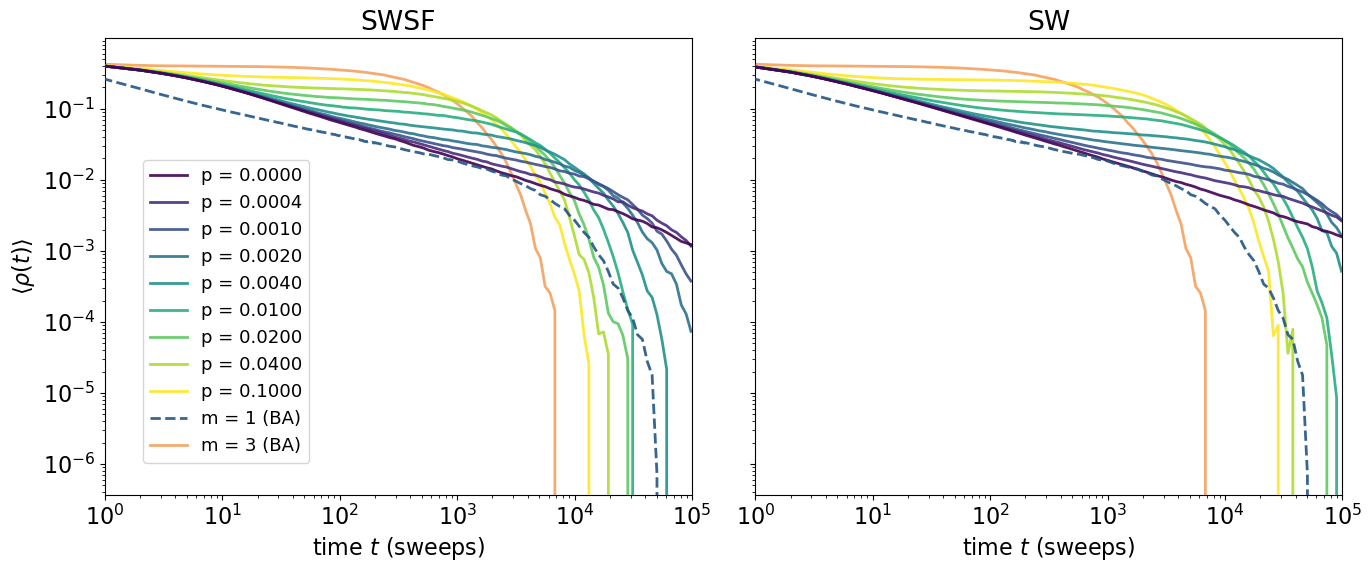
\includegraphics[width=15.5cm,keepaspectratio]{images/SWSFvsSWvsBA_plot.png}
  \caption{Time evolution of the interface density for $N=4000$, averaged over $200$ realizations of the dynamics and $12$ graph realizations, $<k> = 6$ except for BA $m=1$.}
  \label{fig:yourlabel}
\end{figure}

The BA network ($m=3$) has an effective dimension $d=\infty$, consistently, the ordering process stops to reach a metastable state, however, given the finite size of the system, a finite fluctuation can bring it to one of the absorbing states, this is reflected in the late stage exponential decay, giving a finite lifetime to the plateau.\\
The structured scale free ($p=0$ on the left) has an effective dimension $d\simeq1$ \cite{suchecki2005voter}, and tends to order indefinitely, decaying as a power law with exponent $1/2$ as in one-dimensional regular lattices($p=0$ on the right); both are still affected by finite size induced exponential decay, but it kicks in much later.
The rewiring procedure smoothly interpolates between $d=1$ and $d=\infty$: as $p$ increases, the pre-plateau transient shortens and the plateau value itself grows. Degree homogeneity only extends the lifetime of the disordered phase.\\
Up to this point, \emph{effective dimension} has not been rigorously defined, but there are two options: the topological dimension (Hausdorff) or the spectral dimension. The behavior of the $m=1$ (dashed) BA suggests that the relevant concept of dimensionality is indeed the spectral dimension, in fact, $\rho$ tends to zero even if the topological dimension is $d=\infty$, but $d_s = 4/3 <2$ \cite{burda2001statistical}, this is consistent with the idea that the interface edges are performing a random walk in the line graph L(G) and annihilating upon contact \footnote{This is just a naive idea, a more accurate statement would be that the interface edges perform a parity-preserving branching-annihilating random walk (BARW) on L(G).}.

\section{Introducing noise}
Setting $a>0$ in \ref{updateprob} removes the presence of the two absorbing states, since even in full consensus, there is always the possibility of a spontaneous transition, this fact alone changes the universality class of the system \cite{livi2017nonequilibrium}.

\begin{figure}[htbp]
\label{fig:vm comparison}
  \centering
  \includegraphics[width=15cm,keepaspectratio]{images/NoisyVM_p0_p01.png}
  \caption{Time evolution of the interface density for SWSF,$N=4000$, averaged over $200$ realizations of the dynamics and $12$ graph realizations, $<k> = 6$.}
  \label{fig:yourlabel}
\end{figure}

Noise generates mixed states which correspond to a plateau in the mean interface density, if the plateau value is reached before the fast exponential drop, the system becomes insensitive to finite size effects\footnote{ Fine-tuning $a$ could indefinitely sustain an otherwise short-lived plateau.}. The plateau value is still an increasing function of $p$, indicating a collaborative effect between noise and spectral dimension.
At low $a$, the temporal variance grows, reflecting a competition between noise and finite-size effects.
Indeed, a finite-size induced phase transition is found between a unimodal and a bimodal phase, i.e. the system either is in a constant mixed state or the vast majority or nodes are either in one of the two states. This does not fully answer the high variance observed in $\langle \rho (t)\rangle$, because that trajectory was an average over both the dynamics and the different graphs, and because the high oscillations occur at noise values lower than the observed critical value. Although $a_{crit} \to 0$ for $N\to \infty$, it would be interesting to relate $a_{crit}$ to the spectral dimension of the underlying network. 
\begin{figure}[htbp]
  \centering
  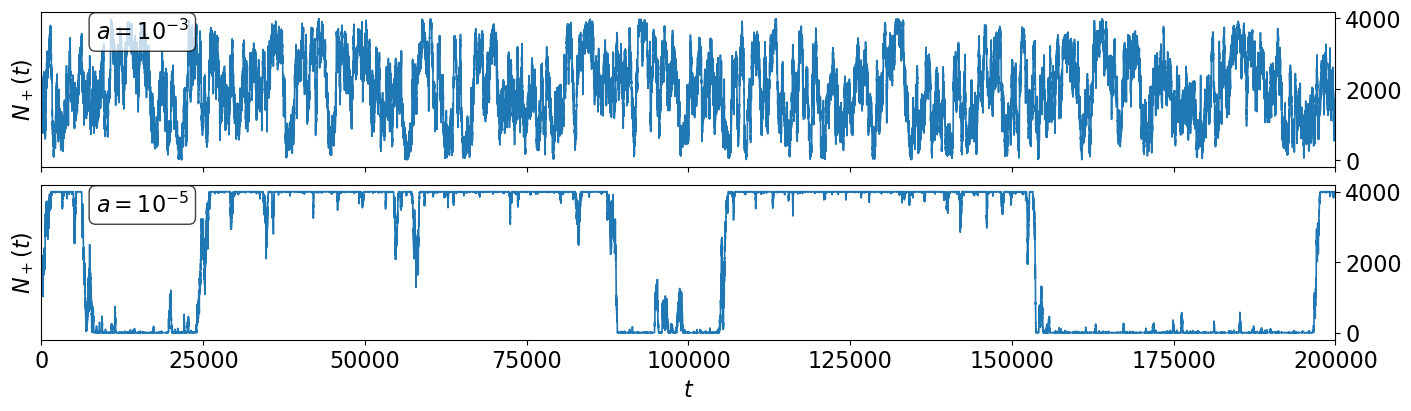
\includegraphics[width=15cm,keepaspectratio]{images/finite_size_noise.png}
  \caption{Single run plot of the number of up-spins for a BA network with $m=2$.}
  \label{fig:yourlabel}
\end{figure}

\newpage
